\chapter{Design}
\label{ch:design}

%
%
% DETECTION
%
%
\section{Detection}

\subsection{Vision sensor} %ASUS camera
The Turtlebot uses The ASUS Xtion PRO LIVE as its vision. Xtion PRO LIVE has two microphones in each side, see figure \ref{fig:asusCamera} nr. 1. Additionally the Xtion PRO LIVE has an RGB camera with a resolution of 640px x 480px at 30 fps, see figure \ref{fig:asusCamera} nr. 3. Furthermore there is a depth camera that has a resolution of 640px x 480px at 30 fps or 320px x 240px at 60 fps, see figure \ref{fig:asusCamera} nr. 2 and 4.
It has a vision distance range from 0.85 m up to 3.5 m and have a field of vision 58° Horizontal, 45° Vertical, 70° Diagonal.
This camera is only for indoor use \ref{ch:CameraRGB}.
\begin{figure}[h]
    \centering
    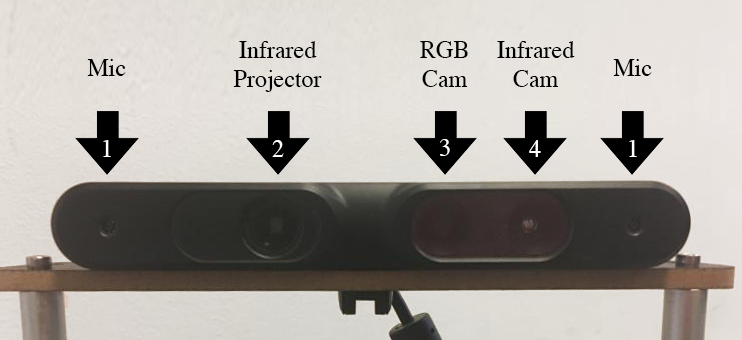
\includegraphics[width=\textwidth]{figures/camera02.png}
    \caption{ASUS Xtion PRO LIVE} 
    \label{fig:asusCamera} 
\end{figure}

%bumber sensor

- Data\\
- Test\\

%
%
% PATH-PLANNING
%
%
\section{Path-planning}

\subsection{Frontier\_Exploration}
Frontier\_Exploration package will be used as a algorithm for our robot to navigate through a perceived environment.\\
The Package provides a costmap\_2D, client/server nodes and Layer BoundedExplorerLayer. The BoundedExplorerLayer can be used for many complex explorations, functioning by two services. Updatepolygonfrontier, this is where the input is telling the robot which area to scan. Then the service GetNextFrontier, will wait for user input and then run the first service again.\\
The robot in this project has no global map, which means the robot should be able to create the map on its own. This can be done autonomously by publishing a starting point, it will then determine its own path and act accordingly. Furthermore, it will still be able to allow user input, such as a published polygons \cite{ROSexploration}.\\

\subsection{ROS}
ROS is used to interact with robots. This operation system comes with a collection of libraries and different commands to execute the communication.\\
The idea with ROS is to connect topics to each other through nodes. On each node there is a topic that you can subscribe or publish to. When there is published or subscribed on a topic it is received in a message that contain the data of this topic. The data can then be used in different programs, to interact with the robot or get information about location and visualization. \\
Before all of this can work there is the need for ROS-master. The ROS-master keeps track of every topic that has been subscribed or published to \cite{ROSwiki}.\\

\subsection{Rviz}
Rviz is a program used by ROS to provide 3D images and point clouds from data given by the robots sensors. Rviz lets the user spectate the robot in different ways. The input the robot gets from cameras and sensors is numbers and coordinates. Rviz converts these numbers into 3D objects which represent these objects\cite{interactiveMarkers}.\\

\subsection{SLAM}
SLAM is not a specific algorithm, but a concept where there are many different approaches. That is why there is different solutions for SLAM. Some are made for indoor use, some for outdoor use.\\
SLAM uses a mapping package \textit{gmapping} in ROS. The gmapping package in ROS is called slam\_gmapping. This package uses data collected from lasers and the robots position to create a 2D map. %Furthermore, slam\_gmapping creates a 2D map in Rviz with lasers and position data collected by the robot.\\
When the robot starts mapping, the localization system AMCL helps the robot to move safely from one location to another.
Information from sensors, such as odometry and gyroscope, is collected when mapping. \\
By comparing data from sensors to the known map, it measures how far it has moved. Moreover, looks at the surrounding area to check its new relative position.\\The robot visualize a map to find the trajectory to move forward. The localization system, AMCL, working-process is described in figure \ref{fig:amcl}.

\begin{figure}
    \centering
    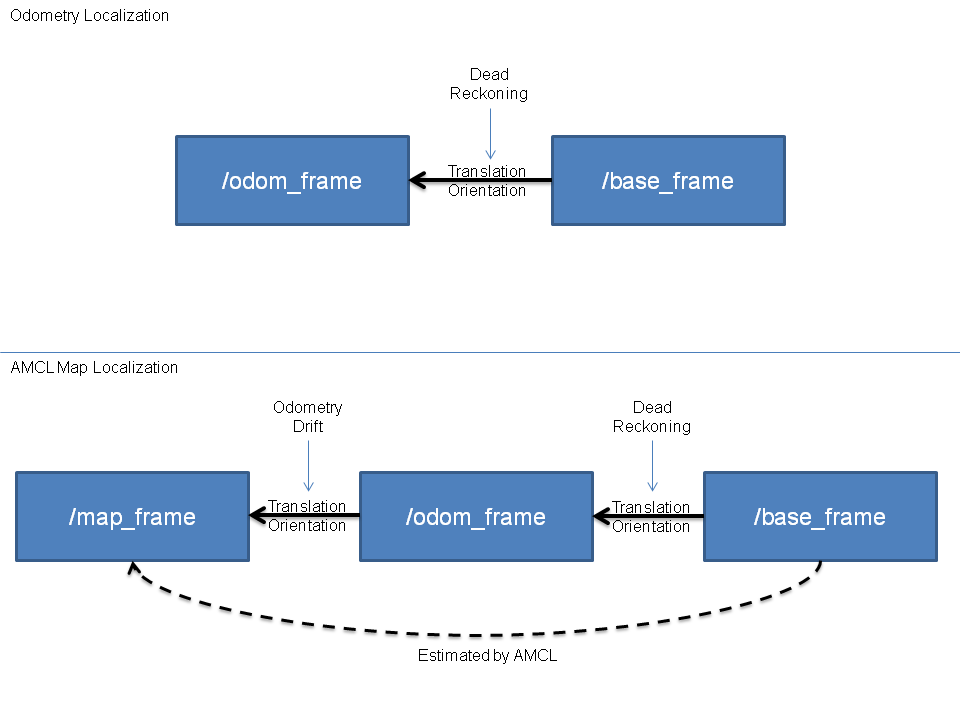
\includegraphics[width=.7\textwidth]{figures/AMCL.png}
    \caption{AMCL working process\cite{AMCL}} 
    \label{fig:amcl} 
\end{figure}

 During operation, AMCL estimates the transformation of the base frame in respect to the global frame. But it only publishes the transformation between the global frame and the odometry frame\cite{AMCL}.\\

- Test

%
%
% MOVEMENT
%
%
\section{Movement}
For control the speed of a DC brushless, there is a need for a motor controller. The controller converts the flat DC power into a squared sin wave, that has the same property's as AC power
- Test